\section{Nos Adaptations}
\subsection{Plugins cssJsLoader, ladpImporter}
\begin{frame}[fragile]{Plugin cssJsLoader}{(steamulo)}
\begin{itemize}
\item Permet de charger nos propres js et css.
\item Personnalisation en fonction du domaine de connexion.
\item Jusqu'en 2022 intégration en \code/iframe/ dans le portail avec \code/postMessage_resize_iframe_in_parent.js/.
\item Depuis 2022 plus d'\code/iframe/, peut-être remplacé par l'utilisation de thème? 
\end{itemize}
\end{frame} 

\begin{frame}{Plugin ldapImporter}{(steamulo)} % some commands, e.g. \verb require [fragile]
\begin{itemize}
\item Est dérivé du plugin ``CAS user and group backend'' de Felix Rupp.
\item Permet l'importation des comptes à partir du ldap
\item Fait l'association des comptes et des groupes aux établissements;
		{\small $$ => table\ etablissement $$} 
\item Filtre et traduit les groupes Grouper en groupes Nextcloud
		{\small $$ => table\ asso\_uai\_user\_group $$ } 
\item Gère les quotas des utilisateurs en fonction des leurs groupes.
\end{itemize}
\end{frame}


\begin{frame}{Plugin ldapimporter} % some commands, e.g. \verb require [fragile]
\begin{figure}
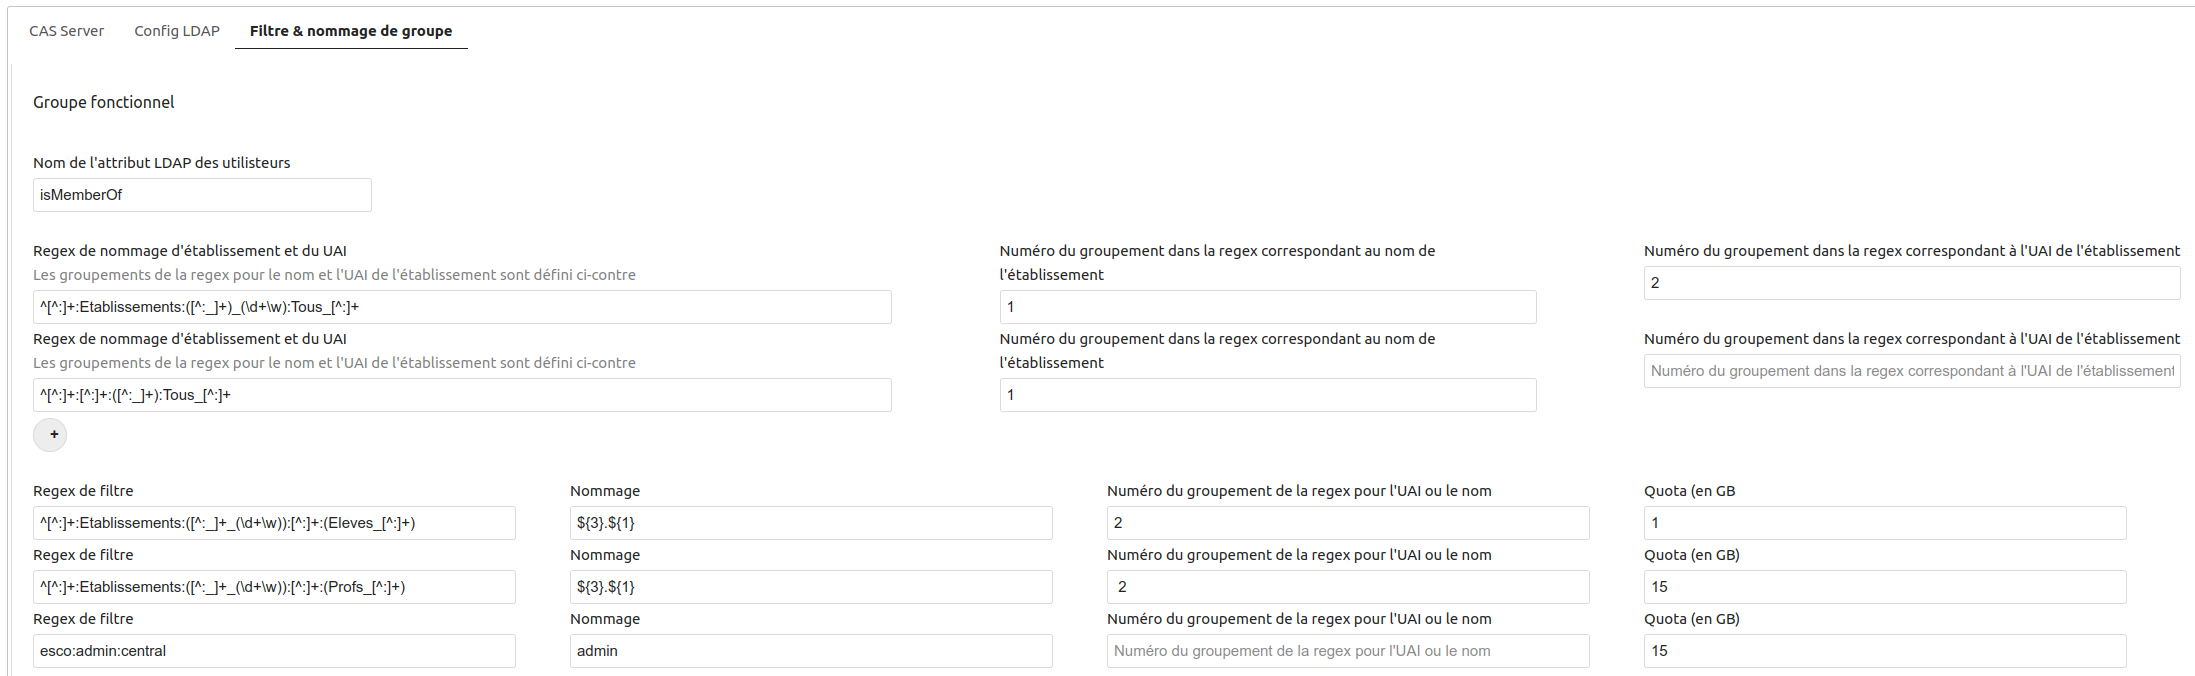
\includegraphics[width=\textwidth, height=0.85\textheight]{ldapimporter.png}
\end{figure}
\end{frame}

\begin{frame}[fragile]{Plugin ldapimporter} % some commands, e.g. \verb require [fragile]
{exemple de filtrage et renommage de groupe}
\begin{list}{}{}
	\item {\tiny Le groupe Grouper :}
\begin{verbatim}
     clg18:Etablissements:ALBERT CAMUS_0180592W:3EME:Eleves_3-2
\end{verbatim}
\item {\tiny satisfait la regex:}
\begin{verbatim}
    ^[^:]+:Etablissements:([^:_]+_(\d+\w)):[^:]+:(Eleves_[^:]+) 
    |   ${3}.${1}  |  2
\end{verbatim}
\item {\tiny est réécrit pour Nexcloud en:}
\begin{verbatim}
    Eleves_3-2.ALBERT CAMUS_0180592W
\end{verbatim}
\item {\tiny et déduit l’appartenance de l'utilisateur à l'établissement}
\begin{verbatim}
    ALBERT CAMUS_0180592W
\end{verbatim}
\end{list}
\end{frame}


\subsection{Plugin files\_sharing}
\begin{frame}[fragile]{Plugin files\_sharing}{Présentation}

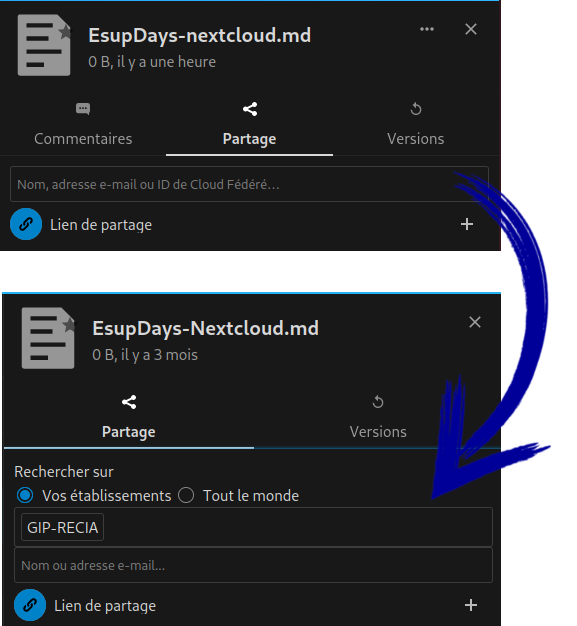
\includegraphics[height=0.75\textheight]{filesharing.png}
\raisebox{3cm}{
\begin{minipage}{8.5cm}
\begin{itemize}
\item Facilité la recherche d'utilisateurs et de groupes pour le partage en permettant la recherche par établissement
\item Fork de l'App File\_sharing de Nextcloud
\item Backend PHP \& frontend Vue JS
\end{itemize}
\end{minipage}
}
\end{frame}

\begin{frame}[fragile]{Plugin files\_sharing}{Utilisation}
\vspace{-20pt}
\begin{figure}
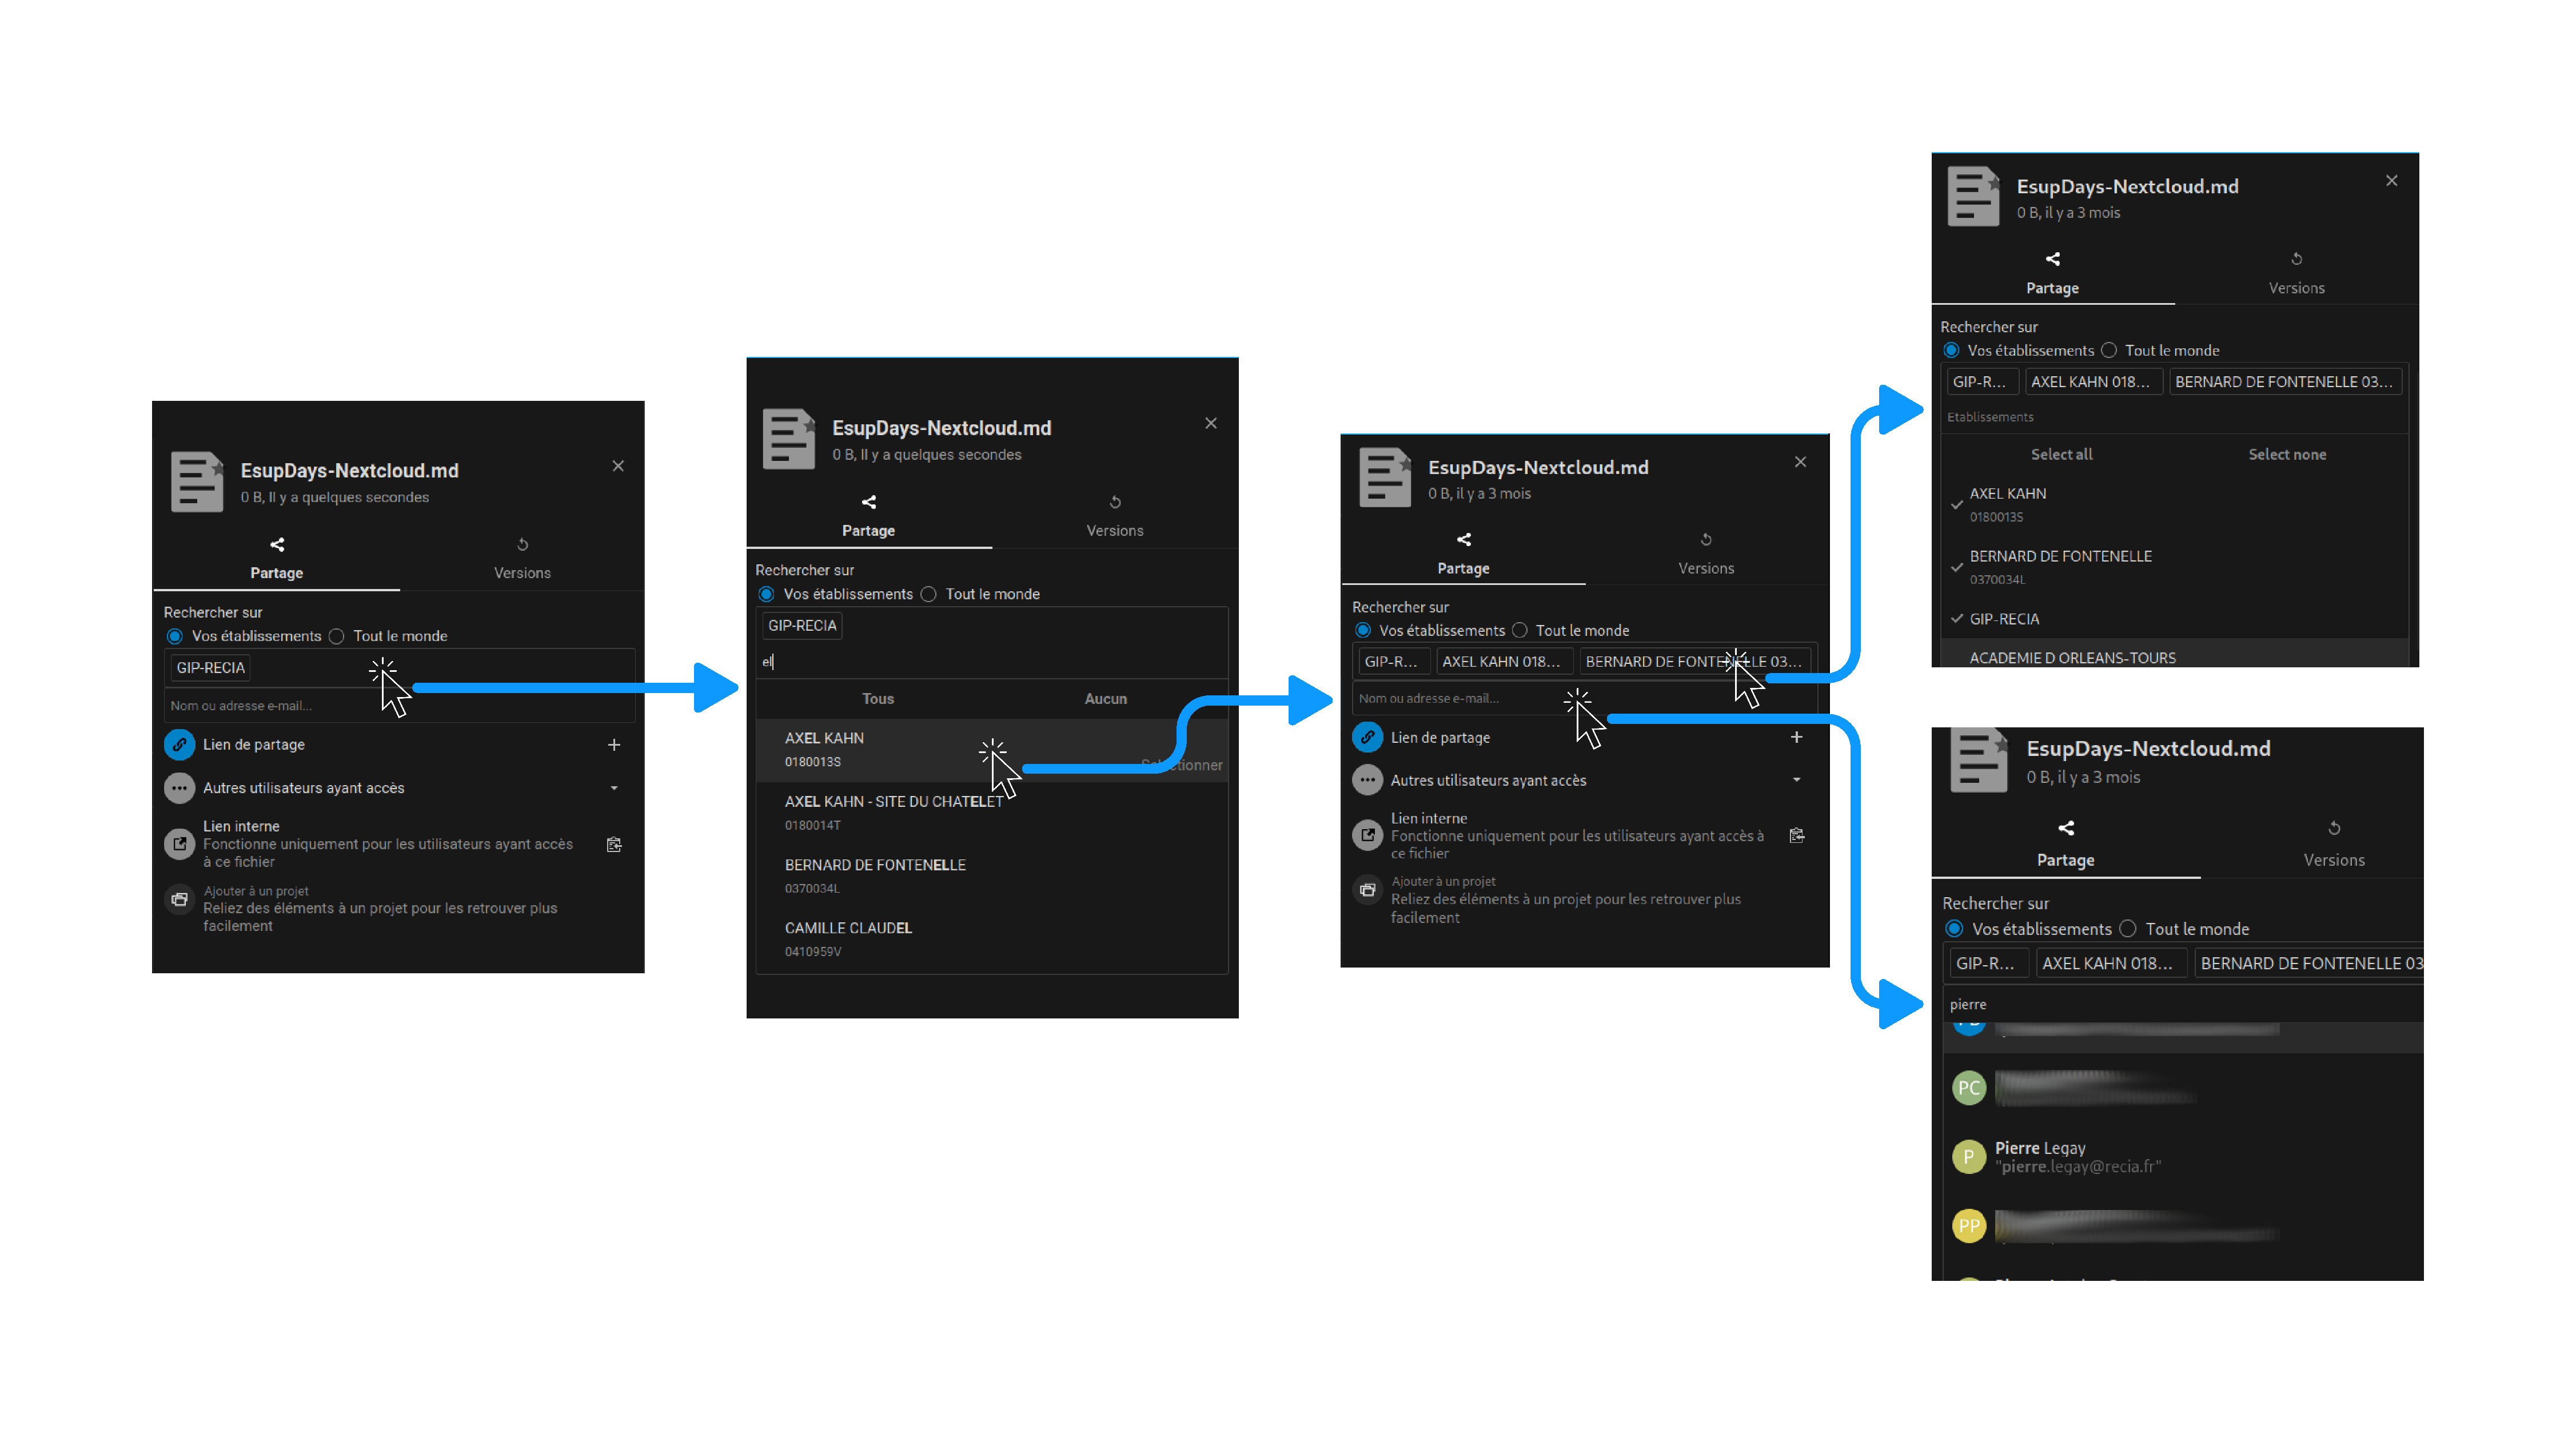
\includegraphics[width=\textwidth]{Fonctionnement-fork-files_sharing.pdf}
\end{figure}
\end{frame}
\begin{frame}[fragile]{Plugin files\_sharing}{Backend}
\begin{itemize}
	\item 2 routes :
		\begin{list}{-}{}
		\item recherche d'établissements liés à l'utilisateur courant
		\item recherche des utilisateurs \& groupes liés à un établissement
		\end{list}
	\item 1 contrôleur
\end{itemize}

\end{frame}

\begin{frame}[fragile]{Plugin files\_sharing}{Frontend}

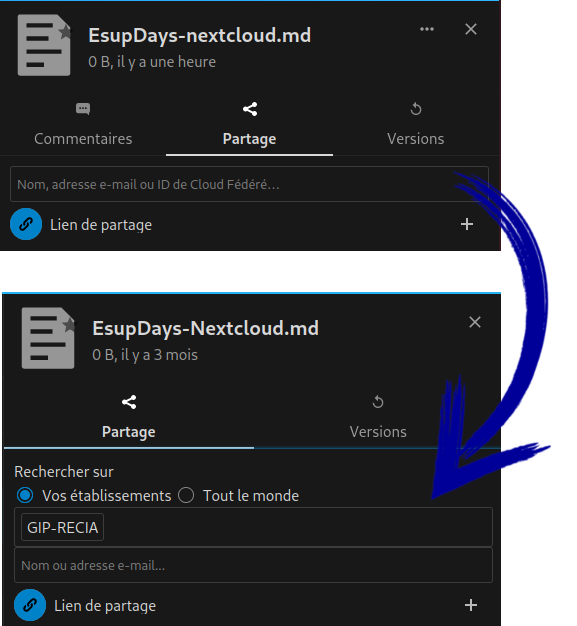
\includegraphics[height=0.75\textheight]{filesharing.png}
\raisebox{3cm}{
\begin{minipage}{8.5cm}
Remplacement dans la vue $SharingTab$ du composant $SharingInput$ par :
\begin{itemize}
\item boutons radios de sélection du type de recherche
\item composant de recherche d'établissement basé sur le composant $NcMultiselect$ 

\item composant dérivé du composant originel $SharingInput$
\end{itemize}
\end{minipage}
}
\end{frame}

\subsection{Bandeau ENT}
\begin{frame}{Bandeau ENT}
Les navigateurs n'acceptant plus le cross-domaine sur les cookies de session (auth CAS).
\begin{itemize}
	\item Création d'un composant web simulant le portail (à la prolongation\_ent)
	\item Intégration dans NC via un thème.
	\item tenant compte du multi-domaines   
\end{itemize}
\end{frame}
